\section{Symmetry}

Define symmetry. Motivate why we care.


\subsection{n-dimensional Cart pole}

So, how can we test a learners ability to detect symmetries and exploit them?
We propose a simple test, the n-dimensional cart pole.

Many people realise that this problem can be reduce to $n$, one dimensional cart pole problems.
But the learner needs to infer that.

\cite{Brockman2016,baselines}

\begin{figure}
\centering
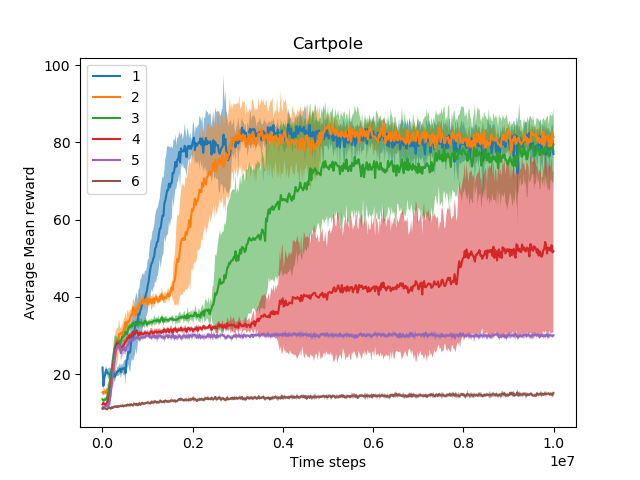
\includegraphics[width=1\textwidth,height=0.5\textheight]{../../pictures/figures/discrete-nd-cart.png}
\caption{PPO2 solving the nd cartpole problem with access to a \textit{Discrete} action space that grows with $2^N$.}
\end{figure}


\begin{figure}
\centering
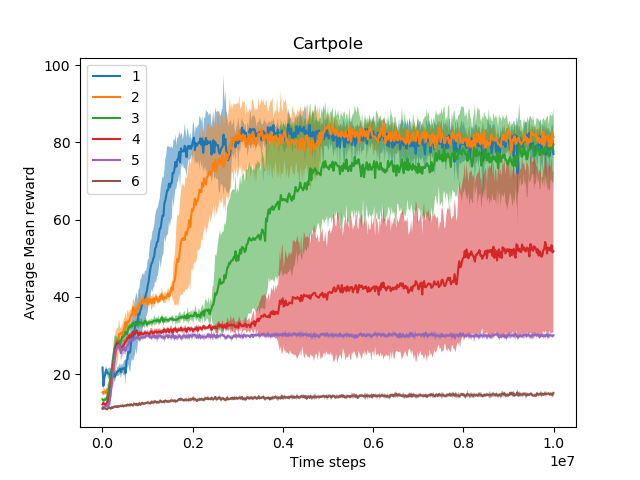
\includegraphics[width=1\textwidth,height=0.5\textheight]{../../pictures/figures/discrete-nd-cart.png}
\caption{PPO2 solving the nd cartpole problem with access to a \textit{MultiBinary} action space that grows with $N$.}
\end{figure}


\subsection{Related work}

relationship to disentanglement.
As recently noted by \cite{Caselles-Dupre2019}, ...
